\section{Rechnermodell}
\label{sec:rechnermodell}

\paragraph{Rechnermodell --- von-Neumann-Rechner}
\begin{figure}[H]
  \centering
  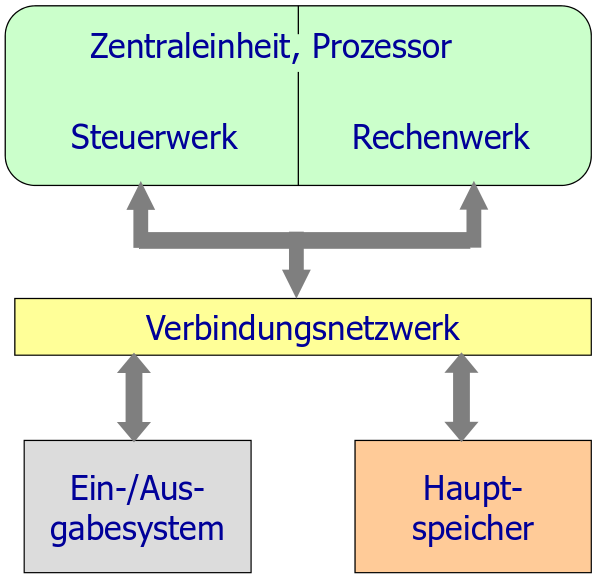
\includegraphics[width=0.33\textwidth]{VonNeumann}
 \label{VonNeumann}
\end{figure}

\paragraph{Von-Neumann-Rechner --- Komponenten}
\begin{items}
	\item \underline{Zentraleinheit}: Verarbeitet Daten gemäß eines Programms
	\begin{enumeration}
		\item \textbf{Leitwerk/Steuerwerk}: Holt Programmbefehle aus Speicher, entschlüsselt sie, steuert Ausführung
		\item \textbf{Rechenwerk/ALU}: Führt arithmetische/logische Operationen aus, wird beeinflussst durch Steuersignale, liefert Meldesignale an Steuerwerk
	\end{enumeration}
	\item \underline{Hauptspeicher}: Besteht aus eindeutig adressierbaren Speicherzellen, bewahrt Programme \emph{und} Daten auf (im Gegensatz zur \emph{Harvard-Architektur})
	\item \underline{Bussystem}:
	\begin{enumeration}
		\item \textbf{Adressleitungen}: Transportieren unidirektional Adressinformationen
		\item \textbf{Datenleitungen}: Transportieren bidirektional Daten und Befehle (von/zum Prozessor)
		\item \textbf{Steuerleitungen}: Transportieren uni- oder bidirektional Steuerinformationen (von/zum Prozessor)
	\end{enumeration}
	\item \underline{Ein-/Ausgabesystem}: Geräte zur Eingabe von Daten/Programmen bzw. zur Ausgabe von Daten (angebunden durch Bussysteme)
\end{items}

\newpage

\paragraph{Rechnermodell --- einfacher Mikroprozessor}
\begin{figure}[H]
  \centering
  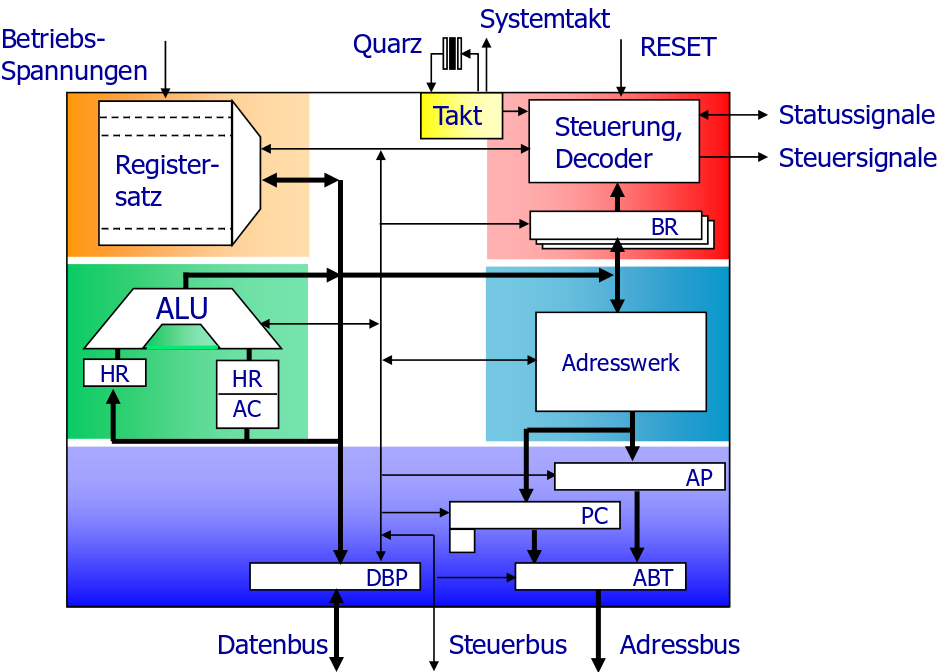
\includegraphics[width=0.33\textwidth]{Mikroprozessor}
  \label{Mikroprozessor}
\end{figure}
\begin{items}
	\item \underline{\textcolor{red!90!black}{Steuerwerk}}: Steuert die Systemkomponenten (meist \emph{dynamisches Schaltwerk} $\leadsto$ Zustandsinformation in Kondensatoren gespeichert $\leadsto$ Refresh-Taktfrequenz erforderlich, sonst Informationsverlust)
	\begin{enumeration}
		\item \textbf{Befehlsregister}: enthält den gerade ausgeführten Befehl (besteht aus mehreren Registern: unterschiedlich lange Befehlsformate bzw. Vorabladen von Befehlen)
		\item \textbf{Decoder}: dekodiert Befehlsworte (= mikroprogrammiertes/festverdrahtetes Schaltwerk)
		\item \textbf{Taktgenerator}: erzeugt Systemtakt (durch externen Quarz), erzeugt ein mit Prozessortakt synchronisiertes Rücksetzsignal (startet Initialisierungsroutine des Steuerwerks)
		\item \textbf{Steuerregister}: Ermöglicht Beeinflussung der aktuellen Arbeitsweise des Steuerwerks (Interrupt enable Bit: wird auf Unterbrechungsanforderung am \code{INT}-Eingang reagiert?, User/System Bit: Sind alle Befehle nutzbar oder nur bestimmte?, Trace Bit: Unterbrechungsroutine nach jeder Befehlsausführung starten?, Decimal Bit: Dual oder BCD rechnen?)
	\end{enumeration}
	\item Befehlsausführung:
	\begin{enumeration}
		\item Holphase: nächster Befehl wird in Befehlsregister geladen
		\item Dekodierphase: Decoder ermittelt Startadresse des Mikroprogramms, welches Befehl ausführt
		\item Ausführungsphase: Mikroprogramm führt Befehl aus, indem Signalfolgen an andere Komponenten übermittelt und Meldesignale ausgewertet werden
	\end{enumeration}

	\item \underline{\textcolor{green!60!black}{Rechenwerk}}: Führt vom Steuerwerk verlangte logische/arithmetische Operationen aus (reines Schaltnetz)
	\begin{enumeration}
		\item \textbf{Statusregister}: informiert Steuerwerk über Ablauf des Ergebnisses (Übertrag \code{CF}, Hilfsübertrag \code{AF}, Null \code{ZF}, Vorzeichen \code{SF}, Überlauf \code{OF}, Even \code{EF}, Parität \code{PF})
		\item \textbf{Hilfsregister/Akkumulatoren}: Zwischenspeichern von Operanden und Ergebnissen (meist zweigeteilt: Akkumulator-Register \code{AC} + nachgeschaltetes Hilfsregister \code{HR} (Latch))
		\item \textbf{Busse}: 2 Eingangsbusse (Operanden), 1 Ausgangsbus (Ergebnis)
		\item \textbf{Ergebnisse}: Werden entweder in Prozessor-Registern gespeichert, zu ALU-Eingangsregistern zurückgeführt oder über externen Datenbus an andere Systemkomponenten übergeben
	\end{enumeration}
	\item Varianten:
	\begin{enumeration}
		\item \textbf{Variante A}: Hilfsregister des Akkumulators hinter der ALU (Vorteil: ALU-Operationen ohne Akkumulatorveränderung möglich. Nur bei alten 8 Bit-Prozessoren)
		\item \textbf{Variante B}: Rechenwerk ohne Akkumulator - Akkumulator in Prozessor-Registersatz verlegt (Vorteil: Mehrere Register können Akkumulatorfunktionen übernehmen. Bei allen modernen 16/32 Bit-Prozessoren)
	\end{enumeration}

	\newpage

	\item Operationen:
	\begin{enumeration}
		\item Arithmetische Operationen (Addieren/Subtrahieren ohne/mit Übertrag, Inkrementieren/Dekrementieren, Multiplizieren/Dividieren ohne/mit Vorzeichen, Komplement)
		\item Logische Verknüpfungen (Negation, Und, Oder, Antivalenz)
		\item Schiebe-/Rotationsoperationen (Links-/Rechts-Verschieben, Links/Rechts ohne/mit Übetragsbit rotieren)
		\item Transportoperationen (Transferieren: move, load, store,\dots)
	\end{enumeration}

	\item \underline{\textcolor{orange}{Registersatz}}: Zwischenspeicherung von häufig benutzten Operanden $\leadsto$ schnellerer Zugriff als auf Hauptspeicher
	\begin{enumeration}
		\item \textbf{Dual-Port-Speicher} zwischen Ein- und Ausgangsbus \\* $\leadsto$ ein Register lesen und anderes schreiben gleichzeitig möglich
		\item \textbf{Zusatzfunktionen}: Inkrementieren, Dekrementieren, Nullsetzen, Inhaltsverschiebung
		\item \textbf{Datenregister}: Zwischenspeichern von Operanden, bei modernen Prozessoren mehrere Datenregister als Akkumulator nutzbar
		\item \textbf{Adressregister}: Speichern von Adressen/-teilen eines Operanden, Basisregister (enthält Anfangsadresse eines Speicherbereichs, unverändert während dessen Bearbeitung), Indexregister (enthält Offset zu Basisadresse zur Auswahl eines bestimmten Datums im Speicherbereich)
		\item \textbf{Spezielle Register}: Instruction pointer, Steuerregister, Statusregister, Interrupt-Behandlungsregister, Stackregister
		\item \textbf{Registerskalierung}: Je nach aktueller Datenlänge (1 Byte, 2 Byte,...) wird Indexregister vor Auswertung mit 1,2,... multipliziert (Vorteil: bessere Registerbreitenausnutzung, da Register nur um 1 de-/inkrementiert werden muss)
		\item \textbf{Laufzeitstack}: LIFP-Speicher im Hauptspeicher, speichert Prozessorstatus und Programmzähler bei Unterprogrammaufruf/Unterbrechungsroutinen, Parameterübergabe, kurzzeitige Datenlagerung bei Ausführung, Datenübertragungsbefehle \code{PUSH} und \code{POP/PULL}
	\end{enumeration}
	\begin{figure}[H]
	  \centering
	  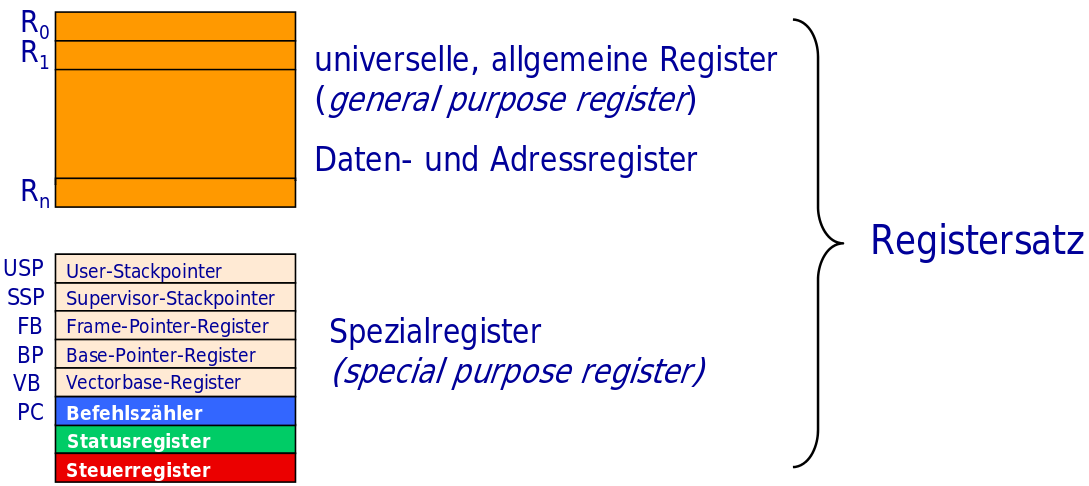
\includegraphics[width=0.33\textwidth]{Registersatz}
	  \label{Registersatz}
	\end{figure}

	\item \underline{\textcolor{ProcessBlue}{Adresswerk}}: Berechnet nach Steuerwerkvorschriften Adresse eines Befehls/Operanden (früher Bestandteil des Rechenwerks, heute sehr komplex, da es viele verschiedene komplexe Adressierungsarten gibt)

	\item Aufbau und Funktionsweise:
	\begin{items}
		\item \textbf{Adress-Addierer - Eingang A}: Registersatz (Adresse aus Basis-/Indexregister), Datenbuspuffer (absolute Adresse im Befehl oder absolute Distanz zu Basisregister)
		\item \textbf{Adress-Addierer - Eingang B}: Befehlszähler (Adresse des aktuellen Befehls), Adresspuffer (Adresse des aktuellen Operanden)
		\item Adressberechnung parralel zu Rechenwerkaktivitäten durch Pipelining
		\item Tätigt Adressrechnung zur virtuellen Speicherverwaltung
		\item Früher separat, heute in Prozessor integriert
		\item Komplexe Adresswerke zur virtuellen Speicherverwaltung
	\end{items}

	\item \underline{\textcolor{blue}{Systembus-Schnittstelle}}: Enthält Zwischenspeicherregister zur kurzfristigen Daten-/Adressaufbewahrung (Befehlszähler, Adresspuffer, Datenbuspuffer) und Ein-/Ausgangstreiber

	\item \underline{Spezielle Funktionseinheiten}: Moderne Mikroprozessoren haben Speicherverwaltungseinheit (MMU), Arithmetik-Einheiten, Cache-Speicher,...
\end{items}

\newpage

\paragraph{Rechnermodell --- CISC}
\begin{items}
	\item = \emph{complex instruction set computer}
	\item \underline{Vorteile}: Mikroprogrammierung begünstigt komplexe Befehle, komplexe Befehle $\leadsto$ kurze Programme, Unterstützung höherer Programmiersprachen durch komplexe Befehle (Abbildung Sprachkonstrukt $\to$ Befehl direkter)
	\item \underline{Fazit}: Entwirklung von Hardware, Programmiersprachen und Einsatzgebieten begünstigt \emph{komplexe} Befehle
	\item \underline{Nachteile}: Umfangreiche Mikroprogramme, verlängerte Entwurfszeit, komplexe Steuerwerke, nur kleine Teile des Befehlssatzes häufig benutzt, größere Fehleranfälligkeit auf Mikroprogrammebene, schwieriger Compilerbau
	\item \underline{80/20-Regel}: Nur 20\% der Befehle werden häufig verwendet
	\item \underline{Cycles per instruction (CPI)}: Bei meisten heutigen CISC-Architekturen: CPI <$>2$
\end{items}

\paragraph{Rechnermodell --- RISC}
\begin{items}
	\item = \emph{reduced instruction set computer}
	\item \underline{Grundprinzipien}:
	\begin{enumeration}
	 	\item Vielbenutzte Befehle so schnell wie möglich machen (keine Mikroprogrammierung, Befehlspipeline)
	 	\item Hauptarbeit durch optimierende Compiler
	 	\item Operanden in großen Registersätzen halten (schneller Zugriff, schnelle Verarbeitung)
	 	\item einheitliche Befehlsformate (schnelle Decodierung)
	 	\item viel Pipelining
	 \end{enumeration}
	\item \underline{Ziele}:
	\begin{enumeration}
		\item Jeder Befehl ein Taktzyklus
		\item alle Befehle gleich lang
		\item nur Load-Store und Register-Register-Befehle (wenige Adressierungsarten $\leadsto$ schnelle Ausführung)
		\item Koprozessorarchitektur für komplexe Befehle
	\end{enumeration}
	\item \underline{keine Ziele}: Unterstützung von Gleitkomma-Arithmetik oder Betriebssystemfunktionen
	\item \underline{Forderungen an RISC-Systeme}: 
	\begin{enumeration}
		\item Mindestens 75\% Ein-Zyklus-Befehle
		\item Länge aller Befehle = Datenbusbreite
		\item Nicht mehr als 128 Befehle
		\item Nicht mehr als 4 Adressierungsarten
		\item Load-Store-Architektur
		\item Festverdrahtete Steuereinheit (keine Mikroprogramme)
		\item Mindestens 32 allgemein verwendbare Register
	\end{enumeration}
\end{items}

\paragraph{RISC --- Prozessoraufbau}
\begin{items}
	\item \underline{Harvard-Architektur}: Programm- und Datenspeicher getrennt $\leadsto$ paralleles Holen von Operanden und Instruktionen
	\item \underline{Varianten}:
	\begin{enumeration}
		\item \textbf{zwei} getrennte Bussysteme bis zu Cachespeichern, nur ein Arbeitsspeicher (niedrigere Kosten)
		\item \textbf{ein} Bussystem (wie Standard-Mikroprozessoren)
	\end{enumeration}
	\item \underline{Systembusschnittstelle}: enthält Registerblocks für Daten und Adressen (parallel Lesen von Daten und Zwischenspeichern von Ergebnis)
	\item \underline{Befehlszähler}: manchmal als Hardware-Stack ausgebildet (schnellere Unterprogrammaufrufe)
	\item \underline{Steuerwerk}: festverdrahtet, Befehlsregister als Warteschlange (FIFO), für jede Pipeline-Stufe ein Register, Opcodes jeder Stufe können von Steuerwerk-Schaltnetz ausgewertet werden
	\item \underline{Registersatz}: große Registeranzahl, erlaubt gleichzeitige Auswahl von 3 bis 4 Registern
	\item \underline{Rechenwerk}: Load/Store-Architektur, Operanden via 2 Operandenbusse aus Registersatz, Ergebnis (im selben Taktzyklus) über Ergebnisbus in Registersatz, keine direkte Verbindung zwischen ALU und Systembus - Transfer über Register
	\item \underline{Superskalarität}: Schafft RISC-Prozessor eine Befehlsausführung pro Takt, so heißt er \emph{superskalar} - pro Takt können mehrere Befehle den Ausführungseinheiten zugeordnet und so viele Befehlsausführungen beendet werden
\end{items}